\documentclass[utf8x, 14pt]{G7-32}

% Настройки стиля ГОСТ 7-32
% Для начала определяем, хотим мы или нет, чтобы рисунки и таблицы нумеровались в пределах раздела, или нам нужна сквозная нумерация.
\EqInChapter % формулы будут нумероваться в пределах раздела
\TableInChapter % таблицы будут нумероваться в пределах раздела
\PicInChapter % рисунки будут нумероваться в пределах раздела
\usepackage{slashbox}

\usepackage[table,xcdraw]{xcolor}

% Добавляем гипертекстовое оглавление в PDF
\usepackage[
bookmarks=true, colorlinks=true, unicode=true,
urlcolor=black,linkcolor=black, anchorcolor=black,
citecolor=black, menucolor=black, filecolor=black,
]{hyperref}

% Изменение начертания шрифта --- после чего выглядит таймсоподобно.
% \usepackage{cyrtimespatched}

% графика
\usepackage{graphicx}
\graphicspath{ {./img/} }

% отделять первую строку раздела абзацным отступом
\usepackage{indentfirst} 

% Пакет Tikz
\usepackage{tikz}
\usetikzlibrary{arrows,positioning,shadows}

% Произвольная нумерация списков.
\usepackage{enumerate}

% ячейки в несколько строчек
\usepackage{multirow}

% itemize внутри tabular
\usepackage{paralist,array}

% объявляем новую команду для переноса строки внутри ячейки таблицы
\newcommand{\specialcell}[2][c]{%
	\begin{tabular}[#1]{@{}c@{}}#2\end{tabular}}

\usepackage{tikz}
\usepackage{pgfplots}
\usepackage{pdfpages}
\usepackage{caption}
% \captionsetup[table]{position=top}
% Листинги

\usepackage{listings}
\usepackage{caption}

\usepackage{courier}
\usepackage{wrapfig}

\usepackage{xcolor}
\captionsetup[lstlisting]{singlelinecheck=off, justification=raggedright}


\definecolor{codegreen}{rgb}{0,0.6,0}
\definecolor{codegray}{rgb}{0.5,0.5,0.5}
\definecolor{codepurple}{rgb}{0.58,0,0.82}
\definecolor{backcolour}{rgb}{0.95,0.95,0.92}


% Значения по умолчанию
\lstset{
  % подсветка синтаксиса
  backgroundcolor=\color{backcolour},   
  commentstyle=\color{codegreen},
  keywordstyle=\color{magenta},
  numberstyle=\tiny\color{codegray},
  stringstyle=\color{codepurple},
  basicstyle= \footnotesize,
  breakatwhitespace=true,% разрыв строк только на whitespacce
  breaklines=true,       % переносить длинные строки
%   captionpos=b,          % подписи снизу -- вроде не надо
  inputencoding=koi8-r,
  numbers=left,          % нумерация слева
  numberstyle=\footnotesize,
  showspaces=false,      % показывать пробелы подчеркиваниями -- идиотизм 70-х годов
  showstringspaces=false,
  showtabs=false,        % и табы тоже
  stepnumber=1,
  tabsize=4,              % кому нужны табы по 8 символов?
  frame=single,
  escapeinside={(*}{*)}, %выделение
  literate={а}{{\selectfont\char224}}1
  {б}{{\selectfont\char225}}1
  {в}{{\selectfont\char226}}1
  {г}{{\selectfont\char227}}1
  {д}{{\selectfont\char228}}1
  {е}{{\selectfont\char229}}1
  {ё}{{\"e}}1
  {ж}{{\selectfont\char230}}1
  {з}{{\selectfont\char231}}1
  {и}{{\selectfont\char232}}1
  {й}{{\selectfont\char233}}1
  {к}{{\selectfont\char234}}1
  {л}{{\selectfont\char235}}1
  {м}{{\selectfont\char236}}1
  {н}{{\selectfont\char237}}1
  {о}{{\selectfont\char238}}1
  {п}{{\selectfont\char239}}1
  {р}{{\selectfont\char240}}1
  {с}{{\selectfont\char241}}1
  {т}{{\selectfont\char242}}1
  {у}{{\selectfont\char243}}1
  {ф}{{\selectfont\char244}}1
  {х}{{\selectfont\char245}}1
  {ц}{{\selectfont\char246}}1
  {ч}{{\selectfont\char247}}1
  {ш}{{\selectfont\char248}}1
  {щ}{{\selectfont\char249}}1
  {ъ}{{\selectfont\char250}}1
  {ы}{{\selectfont\char251}}1
  {ь}{{\selectfont\char252}}1
  {э}{{\selectfont\char253}}1
  {ю}{{\selectfont\char254}}1
  {я}{{\selectfont\char255}}1
  {А}{{\selectfont\char192}}1
  {Б}{{\selectfont\char193}}1
  {В}{{\selectfont\char194}}1
  {Г}{{\selectfont\char195}}1
  {Д}{{\selectfont\char196}}1
  {Е}{{\selectfont\char197}}1
  {Ё}{{\"E}}1
  {Ж}{{\selectfont\char198}}1
  {З}{{\selectfont\char199}}1
  {И}{{\selectfont\char200}}1
  {Й}{{\selectfont\char201}}1
  {К}{{\selectfont\char202}}1
  {Л}{{\selectfont\char203}}1
  {М}{{\selectfont\char204}}1
  {Н}{{\selectfont\char205}}1
  {О}{{\selectfont\char206}}1
  {П}{{\selectfont\char207}}1
  {Р}{{\selectfont\char208}}1
  {С}{{\selectfont\char209}}1
  {Т}{{\selectfont\char210}}1
  {У}{{\selectfont\char211}}1
  {Ф}{{\selectfont\char212}}1
  {Х}{{\selectfont\char213}}1
  {Ц}{{\selectfont\char214}}1
  {Ч}{{\selectfont\char215}}1
  {Ш}{{\selectfont\char216}}1
  {Щ}{{\selectfont\char217}}1
  {Ъ}{{\selectfont\char218}}1
  {Ы}{{\selectfont\char219}}1
  {Ь}{{\selectfont\char220}}1
  {Э}{{\selectfont\char221}}1
  {Ю}{{\selectfont\char222}}1
  {Я}{{\selectfont\char223}}1
}

\lstloadlanguages{
  C++
}

% Стиль для псевдокода: строчки обычно короткие, поэтому размер шрифта побольше
\lstdefinestyle{pseudocode}{
  basicstyle=\small,
  keywordstyle=\color{black}\bfseries\underbar,
  language=Pseudocode,
  numberstyle=\footnotesize,
  commentstyle=\footnotesize\it
}

% Стиль для обычного кода: маленький шрифт
\lstdefinestyle{realcode}{
  basicstyle=\scriptsize,
  numberstyle=\footnotesize
}

% Стиль для коротких кусков обычного кода: средний шрифт
\lstdefinestyle{simplecode}{
  basicstyle=\footnotesize,
  numberstyle=\footnotesize
}

% Стиль для BNF
\lstdefinestyle{grammar}{
  basicstyle=\footnotesize,
  numberstyle=\footnotesize,
  stringstyle=\bfseries\ttfamily,
  language=BNF
}

% Определим свой язык для написания псевдокодов на основе Python
\lstdefinelanguage[]{Pseudocode}[]{Python}{
  morekeywords={each,empty,wait,do},% ключевые слова добавлять сюда
  morecomment=[s]{\{}{\}},% комменты {а-ля Pascal} смотрятся нагляднее
  literate=% а сюда добавлять операторы, которые хотите отображать как мат. символы
    {->}{\ensuremath{$\rightarrow$}~}2%
    {<-}{\ensuremath{$\leftarrow$}~}2%
    {:=}{\ensuremath{$\leftarrow$}~}2%
    {<--}{\ensuremath{$\Longleftarrow$}~}2%
}[keywords,comments]

% Свой язык для задания грамматик в BNF
\lstdefinelanguage[]{BNF}[]{}{
  morekeywords={},
  morecomment=[s]{@}{@},
  morestring=[b]",%
  literate=%
    {->}{\ensuremath{$\rightarrow$}~}2%
    {*}{\ensuremath{$^*$}~}2%
    {+}{\ensuremath{$^+$}~}2%
    {|}{\ensuremath{$|$}~}2%
}[keywords,comments,strings]

% Подписи к листингам на русском языке.
\renewcommand\lstlistingname{\cyr\CYRL\cyri\cyrs\cyrt\cyri\cyrn\cyrg}
\renewcommand\lstlistlistingname{\cyr\CYRL\cyri\cyrs\cyrt\cyri\cyrn\cyrg\cyri}


\pgfplotsset{compat=1.17}
\begin{document}

\frontmatter % выключает нумерацию ВСЕГО; здесь начинаются ненумерованные главы: реферат, введение, глоссарий, сокращения и прочее.

\begin{table}[ht]
	\centering
	\begin{tabular}{|c|p{400pt}|} 
	\hline
		\begin{tabular}[c]{@{}c@{}} 
\includegraphics[scale=0.37]{EmblemBMSTU} \\\end{tabular} &
		\footnotesize\begin{tabular}[c]{@{}c@{}}\textbf{Министерство~науки~и~высшего~образования~Российской~Федерации}\\\textbf{Федеральное~государственное~бюджетное~образовательное~учреждение}\\\textbf{~высшего~образования}\\\textbf{«Московский~государственный~технический~университет}\\\textbf{имени~Н.Э.~Баумана}\\\textbf{(национальный~исследовательский~университет)»}\\\textbf{(МГТУ~им.~Н.Э.~Баумана)}\\\end{tabular}  \\
	\hline
	\end{tabular}
\end{table}
\noindent\rule{\textwidth}{4pt}
\noindent\rule[14pt]{\textwidth}{1pt}
\hfill 
\noindent
\makebox{ФАКУЛЬТЕТ~}%
\makebox[\textwidth][l]{\underline{~~~~«Информатика и системы управления»~~~~~~~~~~~~~~~~~~~~~~~~~~~~~~~~~~~~~~~~~~~~}}%
\\
\noindent
\makebox{КАФЕДРА~}%
\makebox[\textwidth][l]{\underline{~~~~~~~«Программное обеспечение ЭВМ и информационные технологии»~~~~~~~~}}%
\\


\begin{center}
	\vspace{3cm}
	{\bf\huge Отчёт\par}
	{\bf\Large по лабораторной работе № 4\par}
	\vspace{0.5cm}
\end{center}


\noindent
\makebox{\large{\bf Название:}~~~}
\makebox[\textwidth][l]{\large\underline{~Параллельные вычисления~~~~~~~~~~~~~}}\\

\noindent
\makebox{\large{\bf Дисциплина:}~~~}
\makebox[\textwidth][l]{\large\underline{~Анализ алгоритмов~~~~~~~~~~~~~~~~~~~~~~~~~~~~~~~~~~~~~~~~~~~~~~~~~~~~}}\\

\vspace{1.5cm}
\noindent
\begin{tabular}{l c c c c c}
    Студент      & ~ИУ7-52Б~               & \hspace{3.5cm} & \hspace{3.5cm}                 & &  А.С. Пронин \\\cline{2-2}\cline{4-4} \cline{6-6} 
    \hspace{3cm} & {\footnotesize(Группа)} &                & {\footnotesize(Подпись, дата)} & & {\footnotesize(И.О. Фамилия)}
\end{tabular}

\vspace{1cm}

\noindent
\begin{tabular}{l c c c c}
    Преподователь & \hspace{6cm}   & \hspace{3.5cm}                 & & Л.Л. Волкова \\\cline{3-3} \cline{5-5} 
    \hspace{3cm}  &                & {\footnotesize(Подпись, дата)} & & {\footnotesize(И.О. Фамилия)}
\end{tabular}

\begin{center}	
	\vfill
	\large \textit {Москва, 2021}
\end{center}

\thispagestyle {empty}
\pagebreak

\tableofcontents
\pagebreak

\Introduction    
    Многопоточность — способность центрального процессора (CPU) или одного ядра в многоядерном процессоре одновременно выполнять несколько процессов или потоков, соответствующим образом поддерживаемых операционной системой.

    Этот подход отличается от многопроцессорности, так как многопоточность процессов и потоков совместно использует ресурсы одного или нескольких ядер: вычислительных блоков, кэш-памяти ЦПУ или буфера перевода с преобразованием (TLB).
    
    
    В тех случаях, когда многопроцессорные системы включают в себя несколько полных блоков обработки, многопоточность направлена на максимизацию использования ресурсов одного ядра, используя параллелизм на уровне потоков, а также на уровне инструкций.
    
    Поскольку эти два метода являются взаимодополняющими, их иногда объединяют в системах с несколькими многопоточными ЦП и в ЦП с несколькими многопоточными ядрами.
    
    
    Многопоточная парадигма стала более популярной с конца 1990-х годов, поскольку усилия по дальнейшему использованию параллелизма на уровне инструкций застопорились.
    
    Смысл многопоточности — квазимногозадачность на уровне одного исполняемого процесса.
    
    Значит, все потоки процесса помимо общего адресного пространства имеют и общие дескрипторы файлов. Выполняющийся процесс имеет как минимум один (главный) поток.
    
    
    Многопоточность (как доктрину программирования) не следует путать ни с многозадачностью, ни с многопроцессорностью, несмотря на то, что операционные системы, реализующие многозадачность, как правило, реализуют и многопоточность.
    
    
    Достоинства:
    
    \begin{itemize}
    
    	\item облегчение программы посредством использования общего адресного пространства;
    
    	\item меньшие затраты на создание потока в сравнении с процессами;
    
    	\item повышение производительности процесса за счёт распараллеливания процессорных вычислений;
    
    	\item если поток часто теряет кэш, другие потоки могут продолжать использовать неиспользованные вычислительные ресурсы.
    
    \end{itemize}
    
    
    Недостатки:
    
    \begin{itemize}
    
    	\item несколько потоков могут вмешиваться друг в друга при совместном использовании аппаратных ресурсов;
    
    	\item с программной точки зрения аппаратная поддержка многопоточности более трудоемка для программного обеспечения;
    
    	\item проблема планирования потоков;
    
    	\item специфика использования. Вручную настроенные программы на ассемблере, использующие расширения MMX или AltiVec и выполняющие предварительные выборки данных, не страдают от потерь кэша или неиспользуемых вычислительных ресурсов. Таким образом, такие программы не выигрывают от аппаратной многопоточности и действительно могут видеть ухудшенную производительность из-за конкуренции за общие ресурсы.
    
    \end{itemize}
    
    Однако несмотря на количество недостатков, перечисленных выше, многопоточная парадигма имеет большой потенциал на сегодняшний день и при должном написании кода позволяет значительно ускорить однопоточные алгоритмы.
    
    \section*{Цель лабораторной работы}
    Целью данной лабораторной работы является изучение и реализация параллельных вычислений.
    
    \section*{Задачи лабораторной работы}
    \indent В рамках выполнения работы необходимо решить следующие задачи:
    
    \begin{itemize}
    
    	\item изучить понятие параллельных вычислений;
    
    	\item реализовать последовательный и параллельную реализацию подсчета среднего геометрического столюцов матрицы;
    
    	\item сравнить временные характеристики реализованных алгоритмов экспериментально.
    \end{itemize}

\newpage

\mainmatter % это включает нумерацию глав и секций в документе ниже

\chapter{Аналитический раздел}
    \label{cha:analytical}
    \section{Описание задачи}
    Пусть дана прямоугольная матрица
    \begin{equation}
    A_{nm} = \begin{pmatrix}
    a_{11} & a_{12} & \ldots & a_{1m}\\
    a_{21} & a_{22} & \ldots & a_{2m}\\
    \vdots & \vdots & \ddots & \vdots\\
    a_{l1} & a_{l2} & \ldots & a_{lm}
    \end{pmatrix},
    \end{equation}
    
    тогда матрица $B$
    \begin{equation}
    B_{1n} = \begin{pmatrix}
    b_{11} & b_{12} & \ldots & b_{1m}\\
    \end{pmatrix},
    \end{equation}
    
    где
    \begin{equation}
    \label{eq:M}
    B_{1j} = \sqrt[1/n]{\prod_{i=1}^{n} a_{ij}}\quad (j=\overline{1,m})
    \end{equation}
    
    будет называться средним геометрическим столбцов матрицы $A$.
    
    
    В данной лабораторной работе стоит задача распараллеливания алгоритма получения среднего геометрического столбцов матрицы. Так как каждый столбец матрицы $B$ вычисляется независимо от других и матрица $A$ не изменяется, то для параллельного вычисления среднего геометрического, достаточно просто равным образом распределить столбцы матрицы $B$ между потоками.
    
    
    
    \section{Вывод}
    	Обычный алгоритм получения среднего геометрического от ряда чисел в столбце матрицы независимо вычисляет элементы матрицы-результата, что дает большое количество возможностей для реализации параллельного варианта алгоритма.

\newpage
\chapter{Конструкторский раздел}
\label{cha:design}
    На рисунке 2.1 представлена схема обычного алгоритма получения среднего геометрического столбцов матрицы (без распараллеливания). На рисунке 2.2 представлена схема варианта распараллеливания алгоритма получения среднего геометрического столбцов матрицы. На риснуке 2.3 показана схема функции, определяющая границы циклов для каждого из потоков.

    \section{Схемы алгоритмов}
    
    
    \begin{figure}[h]
    	\centering
    	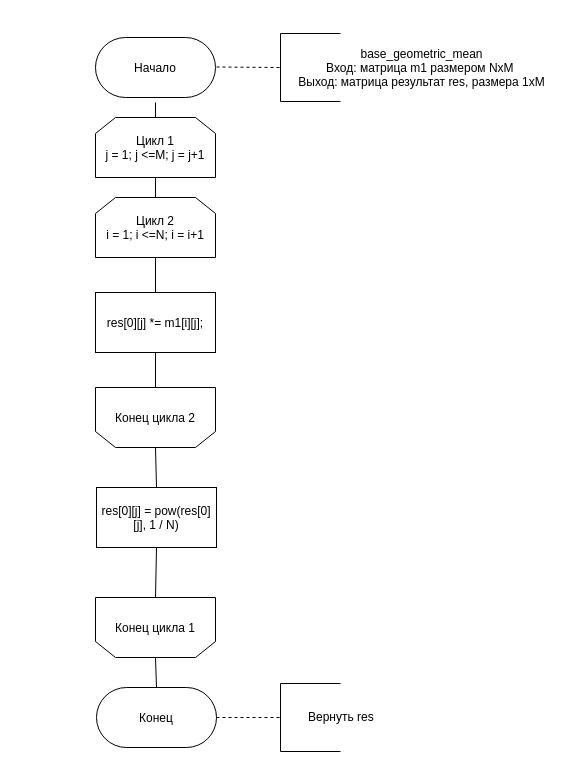
\includegraphics[scale=0.93]{base.jpg}
    	\caption{Схема стандартного алгоритма получения среднего геометрического столбцов матрицы.}
    	\label{fig:mpr}
    \end{figure}
    
    \begin{figure}[h]
    	\centering
    	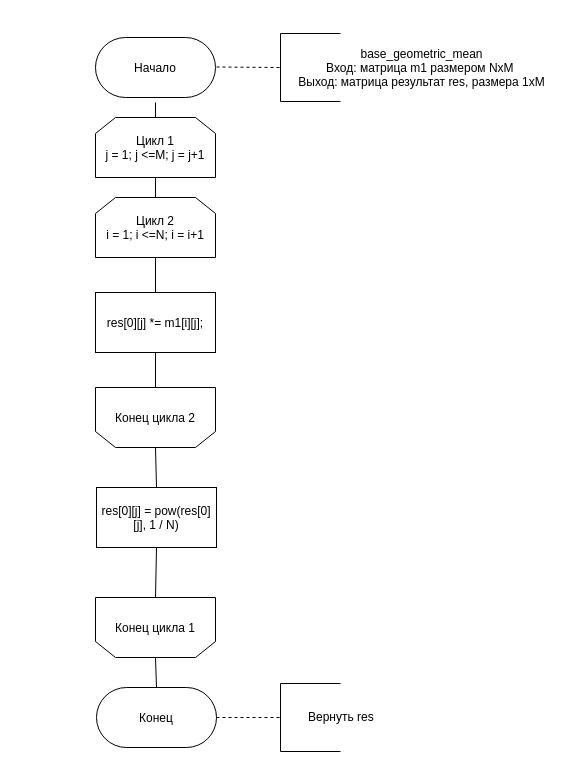
\includegraphics[scale=0.9]{base.jpg}
    	\caption{Схема распараллеленного алгоритма получения среднего геометрического столбцов матрицы.}
    	\label{fig:mpr}
    \end{figure}
    
    \begin{figure}[h]
    	\centering
    	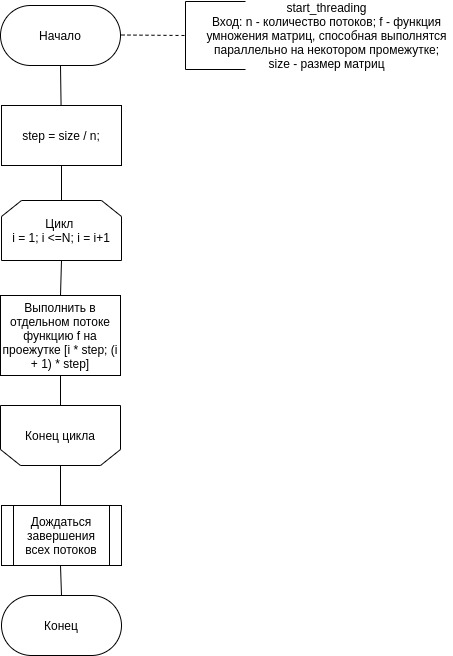
\includegraphics[scale=0.80]{start_threading.jpg}
    	\caption{Функция создания потоков и запуска параллельных реализаций получения среднего геометрического столбцов матрицы}
    	\label{fig:mpr}
    \end{figure}
    
    
    На рисунке 2.4 представленна схема с параллельным выполнением первого цикла
    
    \begin{figure}[h]
    	\centering
    	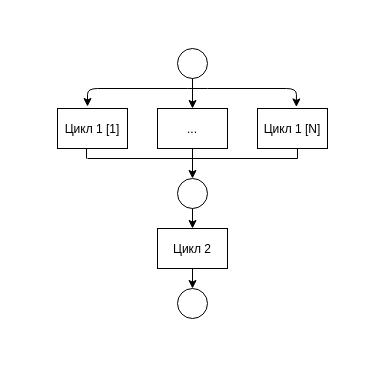
\includegraphics[scale=0.9]{parallel_scheme_01.jpg}
    	\caption{Схема с параллельным выполнением цикла}
    	\label{fig:mpr}
    \end{figure}
    
    
    
    \section{Вывод}
    На основе теоретических данных, полученных из аналитического раздела, была построена схема алгоритма получения среднего геометрического столбцов матрицы, а так же после разделения алгоритма на этапы была предложена схема параллельного выполнения данных этапов.
 

\newpage
\chapter{Технологический раздел}
\label{cha:technological}

    В данном разделе приведены средства реализации и листинги кода.

    \section{Требование к ПО}
    
    К программе предъявляется ряд требований:
    
    \begin{itemize}
    	\item на вход подаются размеры матрицы, а также её элементы;
    	\item на выходе — матрица, которая является результатом получения среднего геометрического столбцов входной матрицы.
    \end{itemize}
    
    \section{Средства реализации}
    Для реализации ПО я выбрал язык программирования Си \cite{C}. Данный выбор обусловлен высокой скоростью работы языка, а так же наличия инструментов для создания и эффективной работы с потоками.
    
    \section{Реализация алгоритмов}
    
    В листингах 3.1 - 3.2 приведена реализация расмотренных ранее алгоритмов получения среднего геометрического столбцов матрицы.
    В листинге 3.3 приведена реализация функции создания и распределения потоков.
    
    \begin{lstlisting}[label=some-code,caption=Функция получения среднего геометрического столбцов матрицы обычным способом, language=C]
    void base_geometric_mean(args_t *args) {
        for (int j = 0; j < M; j++) {
            int ind_tmp_val = 1;
            for (int i = 0; i < N; i++) {
                args->res[ind_tmp_val][j] *= args->m1[i][j];
                if (i % 10 == 0 && i != 0) {
                    double n = N;
                    args->res[ind_tmp_val][j] = pow(args->res[ind_tmp_val][j], static_cast<double>(1) / n);
                    ind_tmp_val++;
                }
            }
            for (int ind = 1; ind < N / 10 + 2; ind++)
                args->res[0][j] *= args->res[ind][j];
        }
    }
    \end{lstlisting}
    
    \begin{lstlisting}[label=some-code,caption=Функция получения среднего геометрического столбцов матрицы параллельно.,language=C]
    void *parallel_geometric_mean_by_columns(void *args) {
        pthread_args_t *all_data = (pthread_args_t *)args;
    
        int col_start = all_data->thread_id * (all_data->matrix_size / all_data->cnt_threads);
        int col_end = (all_data->thread_id + 1) * (all_data->matrix_size / all_data->cnt_threads);
    
        for (int j = col_start; j < col_end; j++) {
            int ind_tmp_val = 1;
            for (int i = 0; i < N; i++) {
                all_data->matrix_container->res[ind_tmp_val][j] *= all_data->matrix_container->m1[i][j];
                if (i % 10 == 0 && i != 0) {
                    double n = N;
                    all_data->matrix_container->res[ind_tmp_val][j] =
                            pow(all_data->matrix_container->res[ind_tmp_val][j], static_cast<double>(1) / n);
                    ind_tmp_val++;
                }
            }
            for (int ind = 1; ind < N / 10 + 2; ind++)
                all_data->matrix_container->res[0][j] *= all_data->matrix_container->res[ind][j];
        }
        return NULL;
    }
    
    \end{lstlisting}
    
    \begin{lstlisting}[label=some-code,caption=Функция создания потоков,language=C]
    int start_threading(args_t *args, const int cnt_threads, const int type) {
        pthread_t *threads = (pthread_t *)malloc(cnt_threads * sizeof(pthread_t));
    
        if (!threads) {
            fprintf(stderr, "Ошибка при выделении памяти. Файл: %s\nСтрока: %d\n", __FILE__, __LINE__);
            return ALLOCATE_ERROR;
        }
    
        pthread_args_t *args_array = (pthread_args_t *)malloc(sizeof(pthread_args_t) * cnt_threads);
    
        if (!args_array) {
            free(threads);
            fprintf(stderr, "Ошибка при выделении памяти: %d\nФайл: %s\n", __LINE__, __FILE__);
            return ALLOCATE_ERROR;
        }
    
        for (int i = 0; i < cnt_threads; i++) {
            args_array[i].matrix_container = args;
            args_array[i].thread_id = i;
            args_array[i].matrix_size = N;
            args_array[i].cnt_threads = cnt_threads;
    
            switch (type) {
                case 1:
                    pthread_create(&threads[i], NULL, parallel_geometric_mean_by_columns, &args_array[i]);
                    break;
            }
        }
    
        for (int i = 0; i < cnt_threads; i++) {
            pthread_join(threads[i], NULL);
        }
    
        free(args_array);
        free(threads);
    
        return OK;
    }
    
    \end{lstlisting}
    
    \section{Тестовые данные}
    
    В таблице~\ref{tabular:test_rec} приведены тесты для функций, реализующих параллельное и обычное умножение матриц. Все тесты пройдены успешно.
    
    \begin{table}[h!]
    	\begin{center}
    		\begin{tabular}{c@{\hspace{7mm}}c@{\hspace{7mm}}c@{\hspace{7mm}}c@{\hspace{7mm}}c@{\hspace{7mm}}c@{\hspace{7mm}}}
    			\hline
    			Матрица & Ожидаемый результат \\ \hline
    			\vspace{4mm}
    			$\begin{pmatrix}
    			1 & 2 & 3 & 4\\
    			4 & 5 & 6 & 5\\
    			7 & 8 & 9 & 6
    			\end{pmatrix}$ &
    			$\begin{pmatrix}
    			3.036589 & 4.308869 & 5.451362 & 4.932424
    			\end{pmatrix}$ \\
    			\vspace{2mm}
    			\vspace{2mm}
    			$\begin{pmatrix}
    			3 & 4 & 2\\
    			27 & 16 & 8
    			\end{pmatrix}$ &
    			$\begin{pmatrix}
    			9 & 8 & 4
    			\end{pmatrix}$ \\
    			\vspace{2mm}
    			\vspace{2mm}
    			$\begin{pmatrix}
    			4
    			\end{pmatrix}$ &
    			$\begin{pmatrix}
    			4
    			\end{pmatrix}$ \\
    			\vspace{2mm}
    			\vspace{2mm}
    			$\begin{pmatrix}
    			0 & 0 & 0\\
    			1 & 2 & 3\\
    			1 & 2 & 3\\
    			1 & 2 & 3
    			\end{pmatrix}$ &
    			$\begin{pmatrix}
    			0 & 0 & 0 & 0
    			\end{pmatrix}$\\
    			\vspace{2mm}
    			\vspace{2mm}
    		\end{tabular}
    	\end{center}
    	\caption{\label{tabular:test_rec} Тестирование функций}
    \end{table}
    
    \section{Вывод}
    
    В данном разделе были разработаны исходные коды алгоритмов: обычный способ умножения матриц и два способа параллельного перемножения матриц.

\newpage
\chapter{Исследовательский раздел}
\label{cha:research}
    
    \section{Технические характеристики}
    
    Ниже приведены технические характеристики устройства, на котором было проведено тестирование ПО:
    
    \begin{itemize}
    	\item Операционная система: Windows 10
    	\item Оперативная память: 36 GB.
    	\item Процессор: Intel Core i7-7700K
    
    \end{itemize}
    
    \section{Время выполнения алгоритмов}
    В таблице 4.1 приведено сравнение реализации параллельного получения среднего геометрического столбцов матрицы с разным количеством потоков при размере исходной матрицы 512. В таблице 4.2 приведено сравнение однопоточной реализации и многопоточных (на четырёх потоках).
    
    \begin{table} [h!]
    	\caption{Таблица времени выполнения параллельных алгоритмов, при размере матрицы 512 (в тиках)}
    	\begin{center}
    		\begin{tabular}{|c c|} 
    			\hline
    			Количество потоков & Паралльная реализация алгоритма \\
    			\hline
    			1 & 16 352 377\\
    			\hline
    			2 & 8 413 109\\
    			\hline
    			4 & 6 617 493\\
    			\hline
    			8 & 5 469 821 \\
    			\hline
    			16 & 5 144 998 \\
    			\hline
    			24 & 5 825 791 \\
    			\hline
    			32 & 7 378 193 \\
    			\hline
    		\end{tabular}
    	\end{center}
    \end{table}
    
    \begin{table} [h!]
    	\caption{Таблица времени выполнения простого и параллельных алгоритмов (на 4 потоках) перемножения матриц (в тиках)}
    	\begin{center}
    		\begin{tabular}{|c c c|} 
    			\hline
    			Размер матрицы & Обычный & Параллельный\\  
    			\hline
    			64 & 209 360 & 766 202 \\
    			\hline
    			128 & 775 438 & 1 057 966 \\
    			\hline
    			256 & 2 575 187 & 2 485 468 \\
    			\hline
    			512 & 10 710 964 & 4 797 693 \\
    			\hline
    			1024 & 60 078 099 & 17 591 850 \\
    			\hline
    		\end{tabular}
    	\end{center}
    \end{table}
    
    \section{Вывод}
    
    Наилучшее время параллельные алгоритмы показали на 16 потоках, что соответствует количеству логических ядер компьютера, на котором проводилось тестирование. На матрицах размером 512 на 512, параллельные алгоритмы улучшают время обычной (однопоточной) реализации перемножения матриц примерно в 2.5 раза. При количестве потоков, большее чем 16, параллельная реализация замедляет выполнение (в сравнении с 16 потоками).
    

\newpage

\backmatter % Здесь заканчивается нумерованная часть документа и начинаются ссылки и
\Conclusion
    В рамках данной лабораторной работы была достигнута её цель: изучены паралелльные вычисления. Также выполнены следующие задачи:

    \begin{itemize}
    	\item было изучено понятие параллельных вычислений;
    	\item были реализованы обычный и  параллельная реализации алгоритма получения среднего геометрического столбцов матрицы;
    	\item было произведено сравнение временных характеристик реализованных алгоритмов экспериментально.
    \end{itemize}
    
    Параллельные реализации алгоритмов выигрывают по скорости у обычной (однопоточной) реализации получения среднего геометрического столбцов матрицы. Наиболее эффективны данные алгоритмы при количестве потоков, совпадающем с количеством логических ядер компьютера. Так, например, на матрицах размером 512 на 512, удалось улучшить время выполнения алгоритма умножения матриц в 2.5 раза (в сравнении с однопоточной реализацией).
% % Список литературы при помощи BibTeX
% Юзать так:
%
% pdflatex report
% bibtex report
% pdflatex report

\bibliographystyle{utf8gost705u}
\bibliography{report}

\end{document}